\lecture{12}{10 April.}{}
\begin{remark}
    The stable matching in \(K_{n, n}\) may not be unique.
\end{remark}

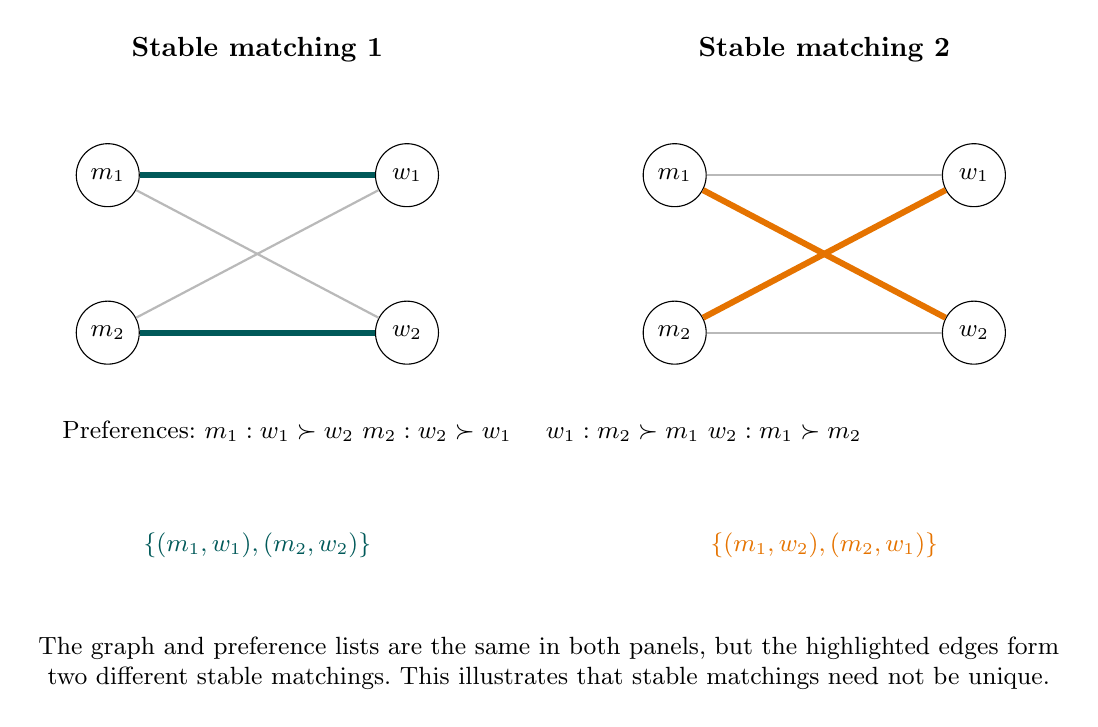
\begin{tikzpicture}[
  person/.style={circle, draw, minimum size=8mm, inner sep=0pt, font=\small},
  every node/.style={font=\small},
  base edge/.style={draw=gray!55, line width=0.8pt},
  matchA/.style={draw=teal!70!black, line width=2.2pt},
  matchB/.style={draw=orange!90!black, line width=2.2pt}
]

% Left panel: first stable matching
\node[font=\bfseries] at (1.9,3.6) {Stable matching 1};

\node[person] (m1a) at (0,2) {$m_1$};
\node[person] (m2a) at (0,0) {$m_2$};
\node[person] (w1a) at (3.8,2) {$w_1$};
\node[person] (w2a) at (3.8,0) {$w_2$};

\draw[base edge] (m1a) -- (w1a);
\draw[base edge] (m1a) -- (w2a);
\draw[base edge] (m2a) -- (w1a);
\draw[base edge] (m2a) -- (w2a);

\draw[matchA] (m1a) -- (w1a);
\draw[matchA] (m2a) -- (w2a);

\node[align=left, anchor=north west] at (-0.7,-1.0) {
  Preferences:\
  $m_1: w_1 \succ w_2$\
  $m_2: w_2 \succ w_1$\ \quad
  $w_1: m_2 \succ m_1$\
  $w_2: m_1 \succ m_2$
};

\node[align=center, text=teal!70!black] at (1.9,-2.7)
  {$\{(m_1,w_1),(m_2,w_2)\}$};

% Right panel: second stable matching
\begin{scope}[xshift=7.2cm]
  \node[font=\bfseries] at (1.9,3.6) {Stable matching 2};

  \node[person] (m1b) at (0,2) {$m_1$};
  \node[person] (m2b) at (0,0) {$m_2$};
  \node[person] (w1b) at (3.8,2) {$w_1$};
  \node[person] (w2b) at (3.8,0) {$w_2$};

  \draw[base edge] (m1b) -- (w1b);
  \draw[base edge] (m1b) -- (w2b);
  \draw[base edge] (m2b) -- (w1b);
  \draw[base edge] (m2b) -- (w2b);

  \draw[matchB] (m1b) -- (w2b);
  \draw[matchB] (m2b) -- (w1b);

  \node[align=center, text=orange!90!black] at (1.9,-2.7)
    {$\{(m_1,w_2),(m_2,w_1)\}$};
\end{scope}

\node[align=center, text width=13cm] at (5.6,-4.2) {
  The graph and preference lists are the same in both panels, but the highlighted edges form two different stable matchings.\
  This illustrates that stable matchings need not be unique.
};

\end{tikzpicture}

\chapter{Connectivity}
\section{Vertex Connectivity}
Recall that a graph \(G\) is connected if there is a path between any two vertices. 

\begin{definition}
    Let \(G = (V, E)\) be a graph. A set \(S \subseteq V\) is a separating set if \(G - S\) is disconnected.   
\end{definition}

\begin{definition}
    The connectivity of a graph, denoted \(\kappa (G)\), is the minimum size of a set \(S \subseteq V\) such that either \(S\) is a separating set or \(G - S\) is a single vertex (only for \(G = K_n\) for the latter case).    
\end{definition}

\begin{definition}
    We say a graph \(G\) is \(k\)-connected if \(\kappa (G) \ge k\).   
\end{definition}

\begin{observation}
    For any \(G\), \(\kappa (G) \le \delta (G)\), where \(\delta (G)\) is the minimum degree of \(G\).     
\end{observation}
\begin{proof}
    For any vertex \(v\), \(S = N(v)\) either disconnects \(v\) from the rest of the graph, or leaves \(v\) as the remaining vertex.    
\end{proof}

\begin{eg}
    \(\kappa (K_{n, m}) = \delta (K_{n, m}) = \min \left\{ n, m \right\} \). 
\end{eg}

\begin{question}
    How many edges does an \(n\)-vertex \(k\)-connected graph have to have?  
\end{question}
\begin{answer}
    For \(k = 2\), the answer is \(n\), since we can consider \(C_n\), and if it has only \(n - 1\) edges, then since it is connected, so it is a tree, but then a tree is \(1\)-connected. 

    For \(k \ge 2\), the answer is \(\left\lceil \frac{kn}{2} \right\rceil \). For the lower bound, since \(\kappa (G) \ge k\), so \(\delta (G) \ge k\). Hence, 
    \[
        e(G) = \frac{1}{2} \sum_{v} \deg(v) \ge \frac{n \delta (G)}{2} \ge \frac{nk}{2}.
    \]
    For the upper bound, \todo{DIY}.         
\end{answer}

\begin{theorem}[Chratal-Erdos, 1972]
    If \(G \neq K_2\) and \(\kappa (G) \ge \alpha (G)\), where \(\alpha (G)\) is the size of largest independent set, then \(G\) is Hamiltonain.
\end{theorem}

\begin{proof}
    Let \(C\) be a largest cycle in \(G\), and let \(\kappa (G) = k\).

    \begin{claim}
        \(\vert C \vert \ge k + 1\).
    \end{claim}

    \begin{explanation}
        Let \(P\) be a maximal path in \(G\) with endpoint \(u\). Since \(P\) is maximal, every neighbor of \(u\) lies on \(P\), so \(N(u) \subseteq V(P)\). Hence
        \[
            \vert N(u) \vert \ge \delta (G) \ge \kappa (G) = k.
        \]
        Let \(v\) be the neighbor of \(u\) furthest along \(P\). Then the subpath of \(P\) from \(u\) to \(v\), together with the edge \(uv\), forms a cycle. Because there are at least \(k\) neighbors of \(u\) on \(P\), this cycle has at least \(k + 1\) vertices.

        \begin{center}
            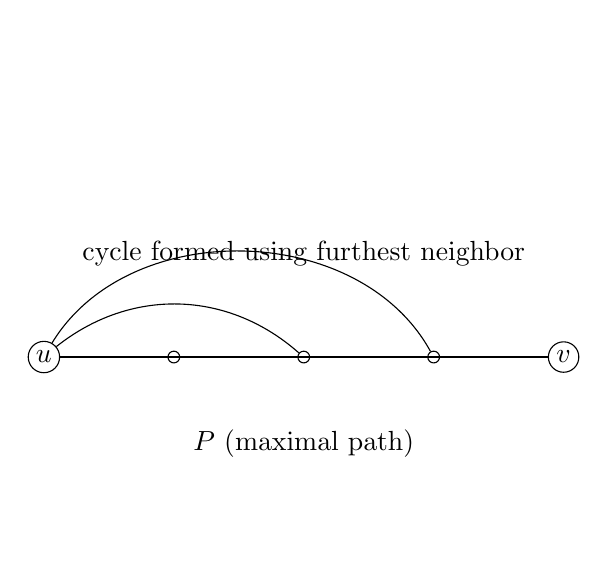
\begin{tikzpicture}[scale=1.1, every node/.style={circle, draw, inner sep=1.5pt}]

            % Path P
            \node (u) at (0,0) {$u$};
            \node (a) at (1.5,0) {};
            \node (b) at (3,0) {};
            \node (c) at (4.5,0) {};
            \node (v) at (6,0) {$v$};

            \draw (u) -- (a) -- (b) -- (c) -- (v);

            % extra neighbors of u on P
            \draw (u) to[bend left=40] (b);
            \draw (u) to[bend left=60] (c);

            % highlight cycle
            \draw[thick] (u) -- (a) -- (b) -- (c) -- (v) -- (u);

            \node[draw=none] at (3,-1) {$P$ (maximal path)};
            \node[draw=none] at (3,1.2) {cycle formed using furthest neighbor};

            \end{tikzpicture}
        \end{center}
    \end{explanation}

    If \(C\) is Hamilton, then we are done. So assume \(C\) is not Hamilton. Let \(Q\) be a component of \(G - C\). Write \(V(C) = \left\{ v_1, \dots , v_t \right\}\) in cycle order.

    \begin{claim}
        At least \(k\) vertices \(v_i\) have a neighbor in \(Q\).
    \end{claim}

    \begin{explanation}
        Let \(S \subseteq V(C)\) be the set of vertices of \(C\) that have a neighbor in \(Q\). If every vertex of \(C\) lies in \(S\), then \(\vert S \vert = \vert C \vert \ge k + 1\), and in particular \(\vert S \vert \ge k\). Otherwise, \(S\) separates the component \(Q\) from the vertices \(V(C) \setminus S\), because every path from \(Q\) to a vertex of \(C\) with no neighbor in \(Q\) must pass through a vertex of \(S\). Thus \(S\) is a vertex cut, so
        \[
            \vert S \vert \ge \kappa (G) = k.
        \]
        Therefore at least \(k\) vertices of \(C\) have a neighbor in \(Q\).
    \end{explanation}

    Let \(v_{i_1}, v_{i_2}, \dots , v_{i_k}\) be vertices of \(C\) that have a neighbor in \(Q\).

    \begin{claim}
        \(v_{i_j+1}\) has no neighbor in \(Q\) for all \(1 \le j \le k\).
    \end{claim}

    \begin{explanation}

    The figure indicates the key idea: if both \(v_{i_j}\) and \(v_{i_j+1}\) had neighbors in \(Q\), then one could leave \(C\) through \(v_{i_j}\), travel through \(Q\), and return to \(C\) at \(v_{i_j+1}\), producing a cycle longer than \(C\).

    \begin{center}
    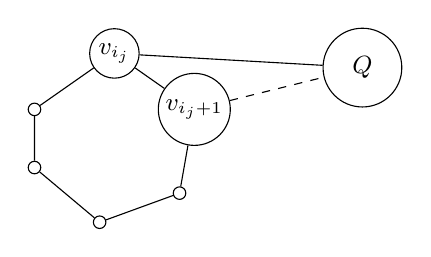
\begin{tikzpicture}[scale=0.45, every node/.style={circle, draw, inner sep=1.6pt, font=\small}]
        \node (v1) at (90:2.4) {$v_{i_j}$};
        \node (v2) at (20:2.4) {$v_{i_j+1}$};
        \node (v3) at (-40:2.4) {};
        \node (v4) at (-100:2.4) {};
        \node (v5) at (-160:2.4) {};
        \node (v6) at (160:2.4) {};
        \draw (v1) -- (v2) -- (v3) -- (v4) -- (v5) -- (v6) -- (v1);

        \node[draw, rounded corners, minimum width=1cm, minimum height=1cm] (Q) at (7,2) {$Q$};
        \draw (v1) -- (Q);
        \draw[dashed] (v2) -- +(Q);
    \end{tikzpicture}
    \end{center}
    \end{explanation}

    \begin{claim}
        \(\left\{ v_{i_j + 1}: 1 \le j \le k \right\}\) is an independent set.
    \end{claim}

    \begin{explanation}
         Assume two vertices \(v_{i_j+1}\) and \(v_{i_\ell+1}\) are adjacent. Since \(v_{i_j}\) and \(v_{i_\ell}\) both have neighbors in the same component \(Q\), there is a path in \(Q\) joining them. Using that path, together with the assumed edge \(v_{i_j+1}v_{i_\ell+1}\) and the appropriate arcs of \(C\), we obtain a cycle that is longer than \(C\). This contradiction shows that no two vertices in \(\left\{ v_{i_j + 1}: 1 \le j \le k \right\}\) are adjacent.

         \begin{center}
            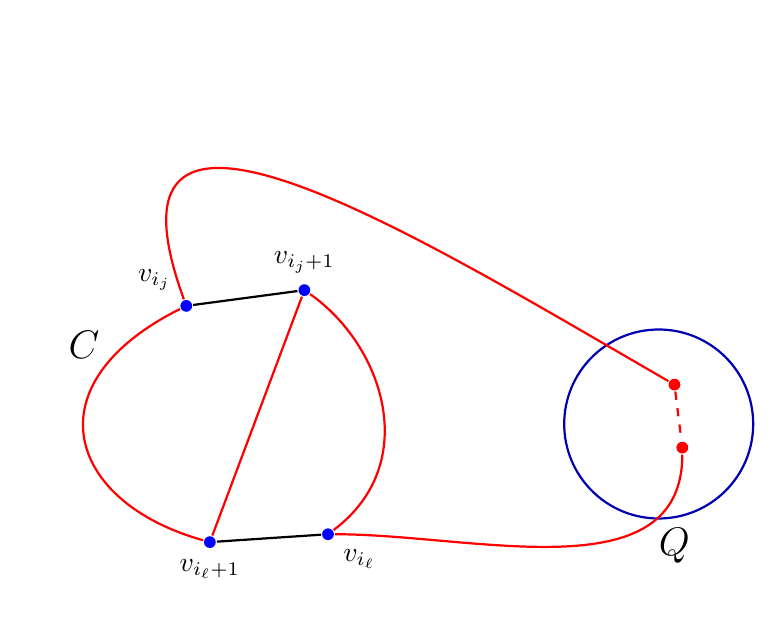
\begin{tikzpicture}[
                node/.style={circle, fill=blue, inner sep=1.5pt},
                rednode/.style={circle, fill=red, inner sep=1.5pt},
                thick
            ]

                % Define main vertices for the cycle C
                \node[node, label=above left:{$v_{i_j}$}] (vij) at (0,3) {};
                \node[node, label=above:{$v_{i_{j}+1}$}] (vij1) at (1.5,3.2) {};
                \node[node, label=below:{$v_{i_{\ell}+1}$}] (vil1) at (0.3,0) {};
                \node[node, label=below right:{$v_{i_{\ell} }$}] (vil) at (1.8,0.1) {};

                % Draw the Cycle C using standard controls (relative curves)
                \draw[red] (vij) .. controls (-2,2) and (-1.5,0.5) .. (vil1);
                \draw[red] (vil) .. controls (3,1) and (2.5,2.5) .. (vij1);
                
                % Draw the straight black edges on the cycle
                \draw[black] (vij) -- (vij1);
                \draw[black] (vil1) -- (vil);
                
                % The internal chord/path
                \draw[red] (vij1) -- (vil1);

                % The Set Q (circle on the right)
                \draw[blue!70!black] (6,1.5) circle (1.2cm);
                \node at (6.2, -0.05) {\Large $Q$};
                
                % Vertices inside Q
                \node[rednode] (q1) at (6.2, 2) {};
                \node[rednode] (q2) at (6.3, 1.2) {};
                \draw[red, dashed] (q1) -- (q2);

                % Paths connecting Cycle C to Q using in/out angles
                \draw[red] (vij) to [out=110, in=150, looseness=1.5] (q1);
                \draw[red] (vil) to [out=0, in=270] (q2);

                % Label for Cycle C
                \node at (-1.3, 2.5) {\Large $C$};

            \end{tikzpicture}
         \end{center}
    \end{explanation}

    Now choose any vertex of \(Q\). Since each \(v_{i_j+1}\) has no neighbor in \(Q\), that vertex is adjacent to none of the vertices in
    \[
        \left\{ v_{i_j + 1}: 1 \le j \le k \right\}.
    \]
    Hence this set, together with any vertex of \(Q\), is an independent set of size \(k + 1\). Thus \(\alpha (G) \ge k + 1 > k = \kappa (G)\), contradicting the assumption \(\kappa (G) \ge \alpha (G)\).

    Therefore \(C\) must be Hamiltonain, and so \(G\) is Hamiltonain.
\end{proof}